\documentclass{template/openetcs_article}
% Use the option "nocc" if the document is not licensed under Creative Commons
%\documentclass[nocc]{template/openetcs_article}
\usepackage{lipsum,url}
\usepackage{booktabs}
\usepackage{multirow}
\usepackage{float}
\usepackage{hyperref}
\graphicspath{{./template/}{.}{./images/}}
\begin{document}
\frontmatter
\project{openETCS}

%Please do not change anything above this line
%============================
% The document metadata is defined below

%assign a report number here
\reportnum{OETCS/WP4/Backlog}

%define your workpackage here
\wp{Work-Package 4: ``Verification and Validation''}

%set a title here
\title{Reduced Set of Parameters for Calculating Braking Curves within 1st Level Verification and Validation}

%set a subtitle here
\subtitle{Version 0.1}

%set the date of the report here
\date{August 2013}

%define a list of authors and their affiliation here

\author{Alexander Nitsch, Benjamin Beichler, Frank Golatowski}

\affiliation{University of Rostock\\ Department of CS and EE
Institute of Applied Microelectronics and CE\\
  Richard-Wagner-Straße 31\\
  18119 Rostock, Germany
   \\eMail:\{alexander.nitsch,benjamin.beichler, frank.golatowski\}@uni-rostock.de }


% define the coverart
\coverart[width=350pt]{openETCS_EUPL}

%define the type of report
\reporttype{Description of work}


\begin{abstract}
%define an abstract here
Work in progress.
\end{abstract}

%=============================
%Do not change the next three lines
\maketitle
\tableofcontents
\listoffiguresandtables
\newpage
%=============================

% The actual document starts below this line
%=============================


%Start here

\section{Reduced Parameter Set of Chapter 3.12 Speed and Distance Monitoring}

University of Rostock proposes only a subset of functions of the SRS, which are part of the current validation model. This is based on the suggestion for model-language evaluation of \href{https://github.com/openETCS/requirements/blob/master/D2.5/D2.5\%20Methods\%20and\%20tools\%20benchmarking\%20methodology.pdf}{WP2}.

Basically in the 1st lvl VnV the emergency brake of a Gamma Train Brake Model is used. This implies that only \texttt{A\_brake\_emergency} and \texttt{T\_brake\_emergency} are used as input from train data to calculate \texttt{A\_safe} and \texttt{T\_be}. Finally these values are used to calculate the \emph{Emergency Deceleration Curve} (EBD) and the Supervision Limits EBI, Warning and Indication.

Further simplifications of the SystemC Model of University of Rostock are currently assumed at the determination of MRSP, since only \emph{Static Speed Profile} and  \emph{Axle Load Profile} are used.
 
%Figure

\begin{figure}[htb]
  \centering
  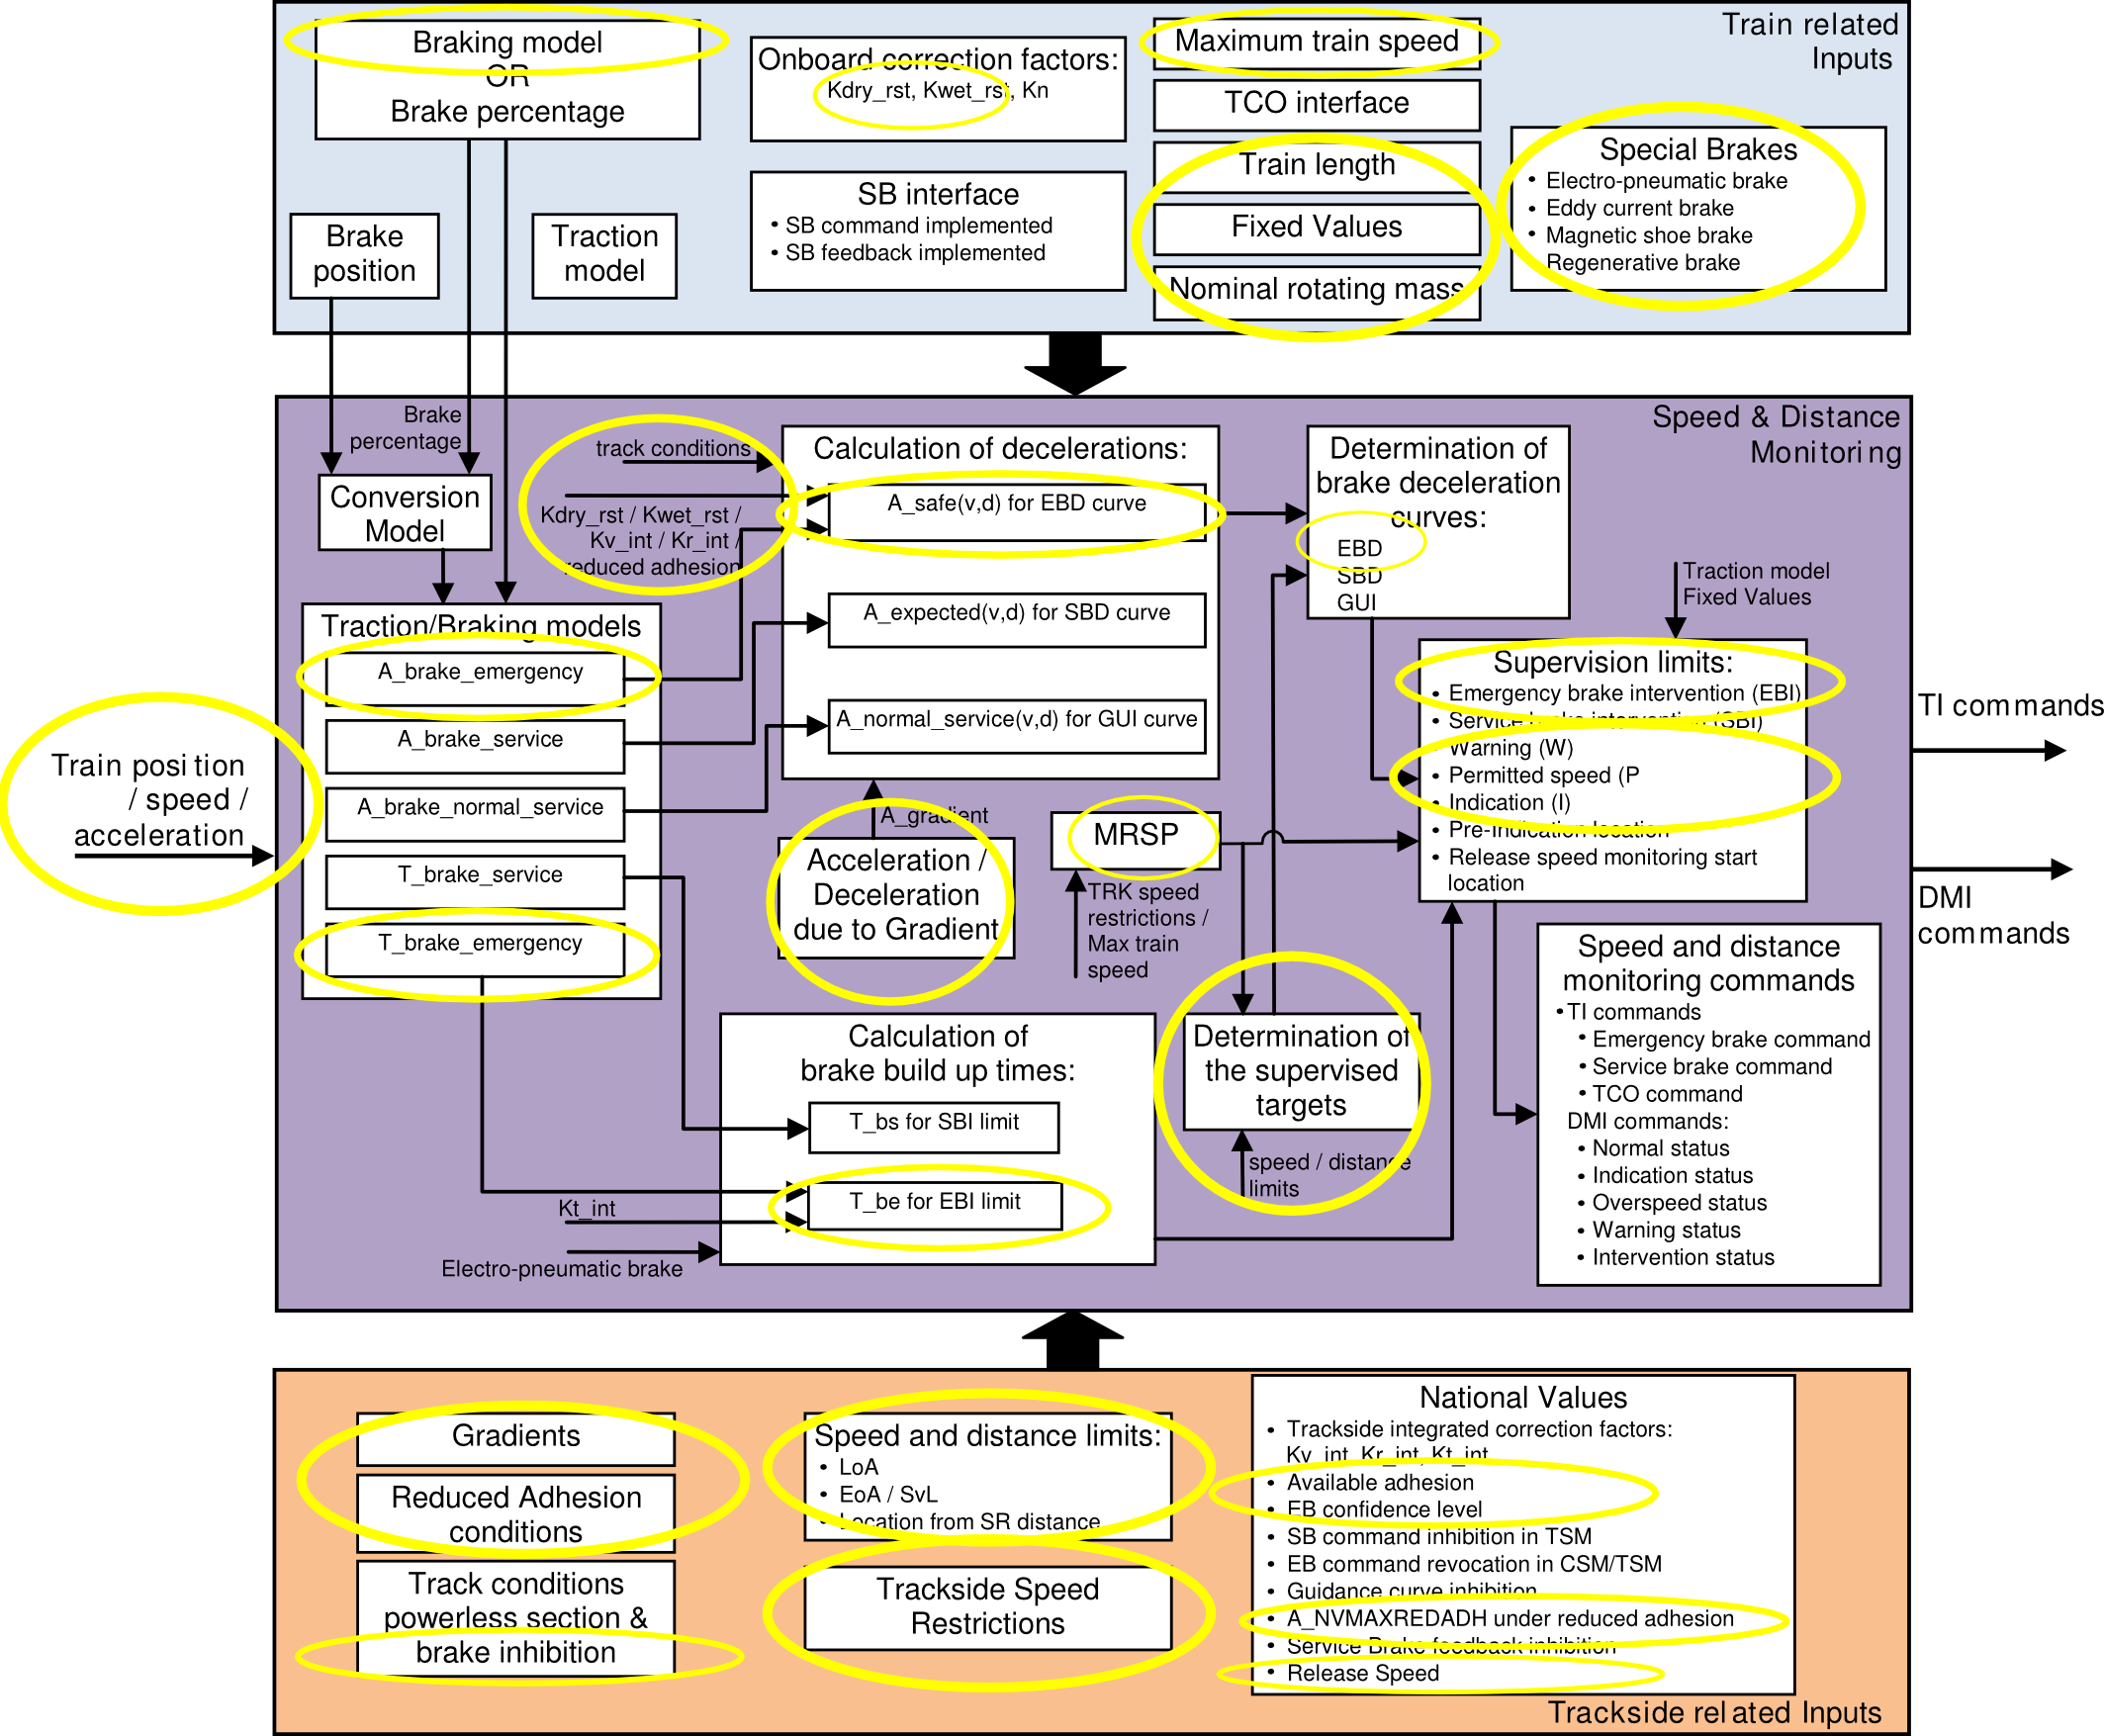
\includegraphics[width=.9\textwidth]{images/reduced_Module_SRS.png}
  \caption{Reduced Module SRS}
  \label{fig:openETCSProcess}
\end{figure}

\section{Required Input Data from Trackside for Calculating Braking Curves}
(extracted from System Requirements Specification Chapter 7 ERTMS/ETCS language)

The Information of following packets are needed for several operations. Caused by the position measurement system and rules of Chapter 3.6 every packet could have a different reference position, because every packet is related to the \emph{Last Relevant Balise Group} (LRBG) of the corresponding message (see chapter 3.8). 

Therefore the Distance Information of all following packets implicitly need to use the same internal reference position system, maybe based on geographical positioning (see chapter 3.6.6) or some other kind of absolute positioning.

Nevertheless in our understanding the problem of different reference locations is out of scope of the Speed and Distance Monitoring.

\begin{table}[H]
\caption{Relevant Packets and inherent Variables - part 1}
\begin{tabular}{|c|p{5cm}|c|c|c|}
\hline 
Packet Number & Packet Name & Variable Name & Page Number \\ 
\hline 
\multirow{10}{*} 3 & \multirow{10}{*} {National Values} & A\_NVMAXREDADH1 & \multirow{10}{*} {11} \\ \cline{3-3} 
 &  & A\_NVMAXREDADH2 &  \\ \cline{3-3}
 &  & A\_NVMAXREDADH3 &  \\ \cline{3-3}
 &  & M\_NVAVADH &  \\ \cline{3-3}
 &  & M\_NVEBCL &  \\ \cline{3-3}
 &  & Q\_NVDRIVER\_ADHES &  \\ \cline{3-3}
 &  & Q\_NVINHSMICPERM &  \\ \cline{3-3}
 &  & Q\_NVKINT &  \\ \cline{3-3}
 &  & Q\_NVKVINTSET &  \\ \cline{3-3}
 &  & V\_NVREL &  \\ \cline{3-3}
\hline 
\multirow{5}{*} {11} & \multirow{5}{*} {Validated train data} & L\_TRAIN & \multirow{5}{*} {39} \\ \cline{3-3} 
 &  & M\_AXLELOADCAT &  \\ \cline{3-3} 
 &  & NC\_CDTRAIN &  \\ \cline{3-3}
 &  & NC\_TRAIN &  \\
\hline
\multirow{4}{*} {12} & \multirow{4}{*} {Level 1 Movement Authority} & Q\_OVERLAP & \multirow{4}{*} {15} \\ \cline{3-3} 
 &  & V\_LOA &  \\ \cline{3-3}
 &  & V\_RELEASEDP &  \\ \cline{3-3}
 &  & V\_RELEASEOL &  \\ \cline{3-3}
\hline 
\multirow{4}{*} {15} & \multirow{4}{*} {Level 2/3 Movement Authority} & D\_DP & \multirow{4}{*} {17} \\ \cline{3-3}
 &  & D\_OL &  \\ \cline{3-3}
 &  & L\_ENDSECTION &  \\ \cline{3-3}
 &  & Q\_DANGERPOINT &  \\ \cline{3-3}
\hline 
\multirow{3}{*} {21} & \multirow{3}{*} {Gradient Profile} & D\_GRADIENT & \multirow{3}{*} {18} \\ \cline{3-3}
 &  & G\_A &  \\ \cline{3-3}
 &  & Q\_GDIR &  \\ 
\hline 
\multirow{7}{*} {27} & \multirow{7}{*} {International Static Speed Profile} & D\_STATIC & \multirow{7}{*} {19} \\ \cline{3-3}
 &  & NC\_CDDIFF &  \\ \cline{3-3}
 &  & NC\_DIFF &  \\ \cline{3-3}
 &  & Q\_DIFF &  \\ \cline{3-3}
\hline 
\end{tabular} 
\end{table}

\begin{table}[H]
\caption{Relevant Packets and inherent Variables - part 2}
\begin{tabular}{|c|p{5cm}|c|c|c|}
\hline 
Packet Number & Packet Name & Variable Name & Page Number \\ 
\hline
\multirow{3}{*} {27} & \multirow{3}{*} {International Static Speed Profile} & Q\_FRONT & \multirow{3}{*} {19} \\ \cline{3-3}
 &  & V\_DIFF &  \\ \cline{3-3}
 &  & V\_STATIC &  \\ \cline{3-3}
\hline 
\multirow{3}{*} {51} & \multirow{3}{*} {Axle load Speed Profile} & D\_AXLELOAD & \multirow{3}{*} {22} \\ \cline{3-3}
 & & L\_AXLELOAD &  \\ \cline{3-3}
 & & V\_AXLELOAD &  \\ \cline{3-3}
\hline 
\multirow{3}{*} {67} & \multirow{3}{*} {Track Condition} & D\_TRACKCOND & \multirow{3}{*} {26} \\ \cline{3-3}
 &  & L\_TRACKCOND &  \\ 
 &  & M\_TRACKCOND &  \\ 
\hline 
\multirow{3}{*} {71} & \multirow{3}{*} {Adhesion Factor} & D\_ADHESION & \multirow{3}{*} {28} \\ \cline{3-3}
 & & L\_ADHESION &  \\ \cline{3-3}
 & & M\_ADHESION &  \\ \cline{3-3}
\hline 
141 & Default Gradient for Temporary Speed
Restriction & G\_TSR & 35 \\ 
\hline 
\end{tabular}
\end{table} 

\section{Train Data and other local Train Variables}

These Variables are part of Train Data and local parts of the EVC (e.g. odometry).

\subsection{Train Data}
\begin{itemize}
\item A\_break\_emergency (for all combinations of special brakes)
\item Kdry\_rst
\item Kwet\_rst
\item L\_TRAIN
\item V\_MAXTRAIN
\item M\_rotating\_nom (rotational mass as fraction of total mass)
\item Binary Status Variables of all Brakes
\item Brake Position (P or G for Person or Freight Trains)
\end{itemize}

\subsection{Odometry and other Sensor Data}
\begin{itemize}
\item $d_{est\,front}$ (estimated front position)
\item $d_{max\,safefront}$
\item $V_{est}$ (estimated speed)
\item $V_{ura}$ (Error in speed measurement)
\item $A_{est1}$ (measured positive Acceleration of Train)

\end{itemize}

\bibliographystyle{unsrt}
%\bibliography{erdc}



%===================================================
%Do NOT change anything below this line

\end{document}
